\documentclass[12pt]{article}

% ============================================================
% Packages
% ============================================================
\usepackage{amsmath, amssymb, amsthm}
\usepackage{mathtools}
\usepackage{booktabs}
\usepackage{graphicx}
\usepackage{hyperref}
\usepackage[utf8]{inputenc}

% ============================================================
% Theorem environments
% ============================================================
\newtheorem{theorem}{Theorem}[section]
\newtheorem{corollary}[theorem]{Corollary}
\newtheorem{lemma}[theorem]{Lemma}
\newtheorem{proposition}[theorem]{Proposition}
\theoremstyle{definition}
\newtheorem{definition}[theorem]{Definition}
\newtheorem{property}[theorem]{Structural Property}
\theoremstyle{remark}
\newtheorem{remark}[theorem]{Remark}

% ============================================================
% Notation
% ============================================================
\newcommand{\RR}{\mathbb{R}}
\newcommand{\ZZ}{\mathbb{Z}}
\newcommand{\CC}{\mathbb{C}}
\newcommand{\kk}{\mathbf{k}}
\newcommand{\LL}{\mathbf{L}}
\newcommand{\nn}{\mathbf{n}}
\newcommand{\Vol}{\mathrm{Vol}}
\DeclareMathOperator{\rank}{rank}
\DeclareMathOperator{\im}{im}
\DeclareMathOperator{\diag}{diag}
\DeclareMathOperator{\tr}{tr}
\DeclareMathOperator{\sgn}{sgn}
\DeclareMathOperator{\cker}{ker}

% ============================================================
% Title
% ============================================================
\title{Exactness-preserving discrete de~Rham complexes\\
under Bloch-periodic boundary conditions}

% Running header (max 75 characters)
% "Exact discrete de Rham complexes under Bloch BCs" = 50 chars
\author{Alexandru Toader\\
Independent researcher, Buz\u{a}u, Romania\\
\texttt{toader\_alexandru@yahoo.com}}
\date{}

\begin{document}
\maketitle

% ============================================================
\begin{abstract}
Discrete exterior calculus (DEC) is often described as free of spurious
modes in the curl--curl eigenvalue problem. We show that this property fails
under Bloch-periodic boundary conditions: the standard discrete curl satisfies
$d_1(\kk)\,d_0(\kk) \neq 0$ for generic wave vector~$\kk$ on any unstructured
polyhedral mesh with faces whose boundary edges carry distinct lattice shifts.
No per-edge phase assignment can restore exactness. We construct an alternative
$d_1(\kk)$ via a face-boundary recurrence that enforces
$d_1(\kk)\,d_0(\kk) = 0$ for all~$\kk$. The construction is explicit, unique
up to per-face gauge, and produces a canonical curl--curl operator with gauge
kernel of dimension~$|V|$. Without exactness, the pollution count equals the
rank excess of~$d_1$ and the Hodge decomposition degrades to random-baseline
hybridization. Experiments on five polyhedral complexes confirm that exactness
eliminates spectral pollution, restores the Hodge splitting, and yields
second-order dispersion convergence. On periodic Voronoi tessellations,
exactness combined with metric isotropy yields
$\omega^2 = |\kk|^2 + O(|\kk|^4)$, verified numerically and supported
by analytical arguments.
\end{abstract}

% ============================================================
\section{Introduction}
\label{sec:intro}
% ============================================================

The discrete exterior calculus (DEC) provides a coordinate-free discretization
of differential forms on cell complexes~\cite{Hirani2003,Desbrun2005}. For
Maxwell's equations on periodic structures, DEC represents the electric field
as a 1-cochain (edge values) and the magnetic flux as a 2-cochain (face values),
with discrete gradient~$d_0$ and curl~$d_1$ acting between cochain spaces. The
curl--curl eigenvalue problem
\begin{equation}\label{eq:curlcurl}
  K\,\mathbf{a} = \omega^2 M\,\mathbf{a}, \qquad
  K = d_1^\dagger \star_2\, d_1, \qquad M = \star_1
\end{equation}
yields electromagnetic eigenfrequencies when the discrete de~Rham sequence
\begin{equation}\label{eq:derham}
  C^0 \xrightarrow{d_0} C^1 \xrightarrow{d_1} C^2
\end{equation}
is exact, i.e., $d_1\,d_0 = 0$. Boffi~\cite{Boffi2010} established that
exactness of the discrete complex is necessary and sufficient for spurious-free
Maxwell eigenvalue computations in the finite element context. The argument
extends to DEC: exactness $d_1 d_0 = 0$ implies $\cker K = \im d_0$ (gauge
completeness), and the positive-definite Hodge star~$\star_2$ ensures discrete
compactness of the physical subspace.

To our knowledge, no construction has been reported that produces an exact
discrete de~Rham complex under Bloch-periodic boundary conditions on
unstructured polyhedral meshes. Unlike standard periodic identification,
Bloch conditions introduce a nontrivial rank-1 local system parametrized
by~$\kk$, so exactness is no longer purely combinatorial---it depends on the
compatibility of phases across face boundaries.

On structured grids (Yee lattice), exactness under Bloch boundary conditions
holds automatically by the tensor-product
topology~\cite{Teixeira1999,Schulz2018,Monkola2023}. The discrete de~Rham
(DDR) method~\cite{DiPietro2020} achieves exactness on polyhedral meshes but
has not been formulated with Bloch periodicity. The FEEC
framework~\cite{Arnold2006,Arnold2010} provides the theoretical foundation for
structure-preserving discretizations but treats simplicial elements, not
polyhedral DEC.

Under Bloch-periodic boundary conditions on unstructured polyhedral meshes, the
standard construction of~$d_1(\kk)$ breaks exactness:
$d_1(\kk)\,d_0(\kk) \neq 0$ for generic~$\kk$. The failure has a combinatorial
origin: faces whose boundary edges carry distinct lattice shifts create
intra-face phase contradictions that no per-edge assignment can resolve.

\paragraph{Contribution} We present:
\begin{enumerate}
  \item A proof that the standard Bloch extension breaks exactness on
    unstructured meshes, and that no per-edge phase fix
    exists~(\S\ref{sec:problem}).
  \item An explicit recurrence construction of an exactness-preserving
    $d_1(\kk)$ that derives curl phases from those in~$d_0(\kk)$
    (\S\ref{sec:construction}, Theorem~\ref{thm:existence}).
  \item Proofs of uniqueness, canonical~$K$, and kernel dimension~$= |V|$
    via K\"unneth formula on~$T^3$ with local
    coefficients~(\S\ref{sec:construction}).
  \item Three structural consequences of inexactness: rank pollution = rank
    excess (algebraic identity), Hodge hybridization at random baseline, and
    trace conservation~(\S\ref{sec:inexactness}).
  \item Identification of Voronoi tessellations as geometries where the exact
    complex yields optimal dispersion $\omega^2 = |\kk|^2 + O(|\kk|^4)$
    (\S\ref{sec:voronoi}).
  \item Verification on five polyhedral complexes including random Voronoi
    meshes with no symmetry~(\S\ref{sec:spectral}, \S\ref{sec:voronoi}).
\end{enumerate}

\paragraph{Viewpoint} The core of the construction is the observation that
Bloch boundary conditions define a rank-1 local system~$\mathcal{L}_\kk$
on~$T^3$, and the discrete operators must form a cochain complex with
coefficients in~$\mathcal{L}_\kk$. The standard DEC approach assigns Bloch
phases independently per edge---this is a discrete connection with nonzero
curvature. Our recurrence derives all phases from~$d_0(\kk)$, producing a flat
connection that preserves exactness. The paper can thus be read as constructing
a flat discrete connection on the Bloch local system such that the twisted
cochain complex remains exact.

\paragraph{Relation to FEEC} In the FEEC
framework~\cite{Arnold2006,Arnold2010}, exactness is preserved via commuting
projections on simplicial subcomplexes. Bloch-periodic twisting introduces a
local system structure not explicitly addressed in existing FEEC
constructions---the standard FEEC machinery handles periodicity by mesh
identification but does not explicitly address the phase consistency required
by nontrivial Bloch parameters. Our construction fills this gap for polyhedral
DEC with diagonal Hodge stars. We do not address the full FEEC program
(commuting projections, approximation theory); the contribution is the
algebraic exactness of the twisted discrete complex.

% ============================================================
\section{Periodic cell complexes and DEC operators}
\label{sec:setup}
% ============================================================

\subsection{Cell complex on the torus}

Let $\Lambda = L_1\ZZ \times L_2\ZZ \times L_3\ZZ$ be a lattice in~$\RR^3$
with fundamental domain $\Omega = [0,L_1) \times [0,L_2) \times [0,L_3)$.
A periodic cell complex $(V, E, F, C)$ on the flat torus
$T^3 = \RR^3/\Lambda$ consists of vertices~$V$, oriented edges~$E$, oriented
faces~$F$, and 3-cells~$C$.

Edges connecting vertices across the periodic boundary carry a lattice shift
vector $\nn_e \in \ZZ^3$:
\begin{equation}\label{eq:shift}
  \nn_e = \mathrm{round}\!\bigl((\mathbf{x}_j - \mathbf{x}_i) / \LL\bigr)
\end{equation}
where division is componentwise. Interior edges have $\nn_e = \mathbf{0}$.

\subsection{Incidence matrices}

The topological gradient $d_0 \in \RR^{|E|\times|V|}$ and curl
$d_1 \in \RR^{|F|\times|E|}$ encode boundary relations:
\begin{equation}\label{eq:d0}
  (d_0)_{ev} = \begin{cases}
    +1 & \text{if } v = \mathrm{head}(e), \\
    -1 & \text{if } v = \mathrm{tail}(e), \\
    \phantom{+}0  & \text{otherwise},
  \end{cases}
\end{equation}
\begin{equation}\label{eq:d1}
  (d_1)_{fe} = \begin{cases}
    +1 & \text{if } e \in \partial f,\ \text{same orientation}, \\
    -1 & \text{if } e \in \partial f,\ \text{opposite orientation}, \\
    \phantom{+}0  & \text{if } e \notin \partial f.
  \end{cases}
\end{equation}
These satisfy $d_1\,d_0 = 0$ (every vertex appears in the boundary of a face
an even number of times with canceling signs).

\subsection{Hodge stars}

The diagonal Hodge star operators
$\star_1 \in \RR^{|E|\times|E|}$ and $\star_2 \in \RR^{|F|\times|F|}$
encode metric information from the dual complex:
\begin{equation}\label{eq:stars}
  (\star_1)_{ee} = \frac{|\sigma^*_e|}{|\sigma_e|}, \qquad
  (\star_2)_{ff} = \frac{|\sigma^*_f|}{|\sigma_f|}
\end{equation}
where $\sigma_e$, $\sigma_f$ are primal edge length and face area, and
$\sigma^*_e$, $\sigma^*_f$ are their dual counterparts. For the SC cubic
lattice with constant~$a$, the stars are uniform:
$\star_1 = a\,I$, $\star_2 = a^{-1}\,I$.

\subsection{Bloch-twisted operators}

For wave vector $\kk \in \RR^3$, the Bloch-twisted gradient acts on
0-cochains~$u$ by:
\begin{equation}\label{eq:d0bloch}
  (d_0(\kk)\,u)_e = e^{i\kk\cdot\nn_e\LL}\,u_{\mathrm{head}(e)}
                   - u_{\mathrm{tail}(e)}.
\end{equation}
When $\nn_e = \mathbf{0}$ (interior edge), this reduces to
$(d_0\,u)_e = u_{\mathrm{head}} - u_{\mathrm{tail}}$.
At $\kk = \mathbf{0}$, $d_0(\kk) = d_0$ (topological gradient).

The standard Bloch curl applies independent per-edge phases:
\begin{equation}\label{eq:d1std}
  d_1^{\mathrm{std}}(\kk)[f,e] = d_1[f,e] \cdot e^{i\kk\cdot\nn_e\LL}.
\end{equation}
This is the construction used in existing DEC-based Maxwell solvers. We show
in~\S\ref{sec:problem} that
$d_1^{\mathrm{std}}(\kk)\,d_0(\kk) \neq 0$ for generic~$\kk$ on unstructured
meshes.

\subsection{Test structures}
\label{sec:structures}

We verify the construction on five periodic polyhedral complexes spanning
three qualitatively different categories (Table~\ref{tab:structures}).

\begin{table}[h]
\centering
\begin{tabular}{llrrrr}
\toprule
Structure & Type & $|V|$ & $|E|$ & $|F|$ & $|C|$ \\
\midrule
SC ($N{=}3$)       & Regular cubic lattice      & 27  & 81  & 81  & 27 \\
Kelvin ($N{=}2$)   & BCC Voronoi tessellation   & 96  & 192 & 112 & 16 \\
C15 ($N{=}1$)      & Laves phase Voronoi        & 136 & 272 & 160 & 24 \\
WP ($N{=}1$)       & A15 Voronoi                & 46  & 92  & 54  & 8  \\
Random Voronoi     & 50 uniform points          & 206--354 & 412--708 & 236--404 & 50 \\
\bottomrule
\end{tabular}
\caption{Test structures. The Voronoi tessellations have 4~edges per vertex
and 3~faces per edge (Plateau structure). Random Voronoi meshes are constructed
from 50 uniformly distributed points on~$T^3$; the range reflects 10~different
seeds.}
\label{tab:structures}
\end{table}

\begin{figure}[h]
\centering
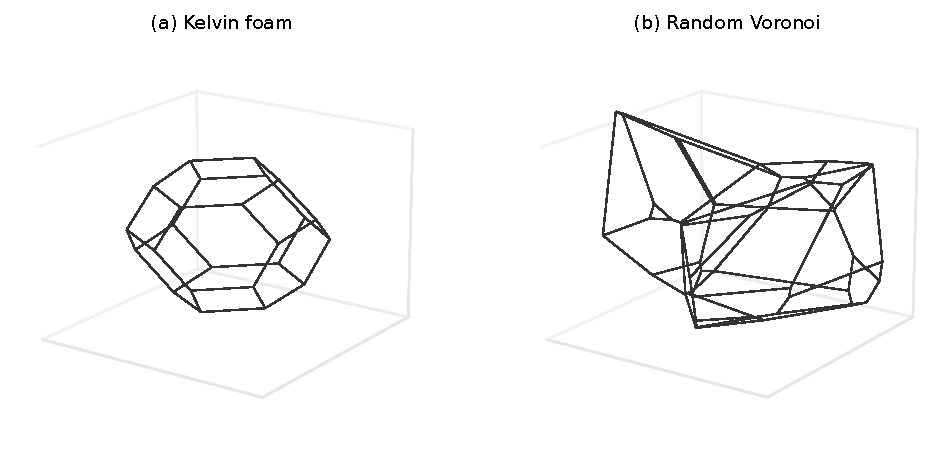
\includegraphics[width=\textwidth]{fig1_meshes.pdf}
\caption{Wireframe view of two test structures (central region of the periodic
box). (a)~Kelvin: regular BCC Voronoi tessellation producing truncated
octahedra with hexagonal and square faces. (b)~Random Voronoi: irregular
polyhedral cells with no lattice symmetry.}
\label{fig:meshes}
\end{figure}

% ============================================================
\section{The exactness problem}
\label{sec:problem}
% ============================================================

\subsection{Standard Bloch curl breaks exactness}

\begin{proposition}\label{prop:break}
If face~$f$ has $\geq 2$ boundary edges with distinct lattice shifts
$\nn_a \neq \nn_b$ sharing a vertex, then
$d_1^{\mathrm{std}}(\kk)\,d_0(\kk) \neq 0$ for all~$\kk$ outside the
hyperplane $\{\kk : e^{i\kk\cdot(\nn_a - \nn_b)\LL} = 1\}$. In particular,
the failure occurs on an open dense set of~$\kk$---it is structural, not
numerical.
\end{proposition}

\begin{proof}
At the shared vertex~$v$, the two contributions to $(d_1 d_0)[f,v]$ carry
phases $e^{i\kk\cdot\nn_a\LL}$ and $e^{i\kk\cdot\nn_b\LL}$. Cancellation
requires $e^{i\kk\cdot(\nn_a - \nn_b)\LL} = 1$, which defines a hyperplane
in~$\kk$-space. This holds at $\kk = \mathbf{0}$ but fails generically when
$\nn_a \neq \nn_b$.
\end{proof}

\begin{table}[h]
\centering
\begin{tabular}{lcrr}
\toprule
Structure & $\|d_1^{\mathrm{std}} d_0\|$ & $n_{\mathrm{spur}}$ [100] & $n_{\mathrm{spur}}$ [111] \\
\midrule
Kelvin $N{=}2$   & 7.54  & 6  & 14 \\
C15 $N{=}1$      & 7.80  & 9  & 16 \\
WP $N{=}1$       & 5.07  & 3  & 7  \\
SC $N{=}3$       & 6.21  & 5  & 13 \\
Random Voronoi   & 10.5--11.7 & 15--19 & --- \\
\bottomrule
\end{tabular}
\caption{Exactness violation and spurious mode count at 10\% of the Brillouin
zone. Direction-dependent pollution: $[100] < [110] < [111]$, universal on all
structures.}
\label{tab:pollution}
\end{table}

\subsection{No per-edge fix exists}

\begin{corollary}\label{cor:noedge}
Let $\varphi\colon E \times \RR^3 \to \CC^*$ be any function assigning a
multiplicative phase to each edge, depending only on the edge---i.e.,
independent of the face context or position along the face boundary.
Define $\tilde{d}_1(\kk)[f,e] = d_1[f,e]\cdot\varphi(e,\kk)$. Then
$\tilde{d}_1(\kk)\,d_0(\kk) \neq 0$ for generic~$\kk$ on any mesh with faces
whose boundary edges carry distinct lattice shifts.
\end{corollary}

More precisely: a per-edge phase $\varphi \in C^1(E; U(1))$ is a 1-cochain,
but exactness requires 2-cochain data---each face determines its own phase
assignment via the recurrence. The obstruction is that the exact phases are
face-dependent, not edge-dependent.

\begin{proof}
By the uniqueness result of \S\ref{sec:construction}
(Corollary~\ref{cor:unique} below), any local $d_1$ with $d_1 d_0 = 0$ has
$d_1[f,:] = \lambda_f \cdot d_1^{\mathrm{ex}}[f,:]$---the phases depend on
the face, not just on the edge. A multiplicative 1-cochain $\varphi(e,\kk)$
assigns the same factor to edge~$e$ regardless of which face it belongs to.
But the recurrence gives $\psi_b/\psi_a = e^{i\kk\cdot\mathbf{S}\LL}$ where
$\mathbf{S} \in \ZZ^3$ is the net lattice shift along the partial boundary
path from position~$a$ to~$b$. When two edges of the same face have the same
lattice shift but different positions in the face boundary, their exact phases
differ by $e^{i\kk\cdot\mathbf{S}\LL} \neq 1$. A 1-cochain multiplicator
cannot produce this face-dependent variation.

\emph{Explicit example.} On Kelvin $N{=}2$, face~1 has three shift-$\mathbf{0}$
edges at positions~0, 2, 4. The recurrence gives
$\psi_2/\psi_0 = e^{-ik_x L} \neq 1$ for $k_x \neq 0$. Out of 112~faces,
37~exhibit such contradictions.
\end{proof}

\paragraph{Numerical demonstration}
Optimizing 192~free edge phases via L-BFGS-B (10~random starts, all converge
to unique global minimum):
\[
  \min_\theta \|d_1(\theta)\,d_0\| = 1.2564
\]
while the recurrence construction (\S\ref{sec:construction}) achieves
$7.86 \times 10^{-16}$. Ratio: $10^{15}$. Per-edge approach is fundamentally
impossible, not merely suboptimal.

\begin{remark}[Extensive pollution]\label{rem:extensive}
The pollution count grows as $n_{\mathrm{spur}} \sim N^{2.3}$ on Kelvin
($N = 2, 3, 4$), between surface~($N^2$) and volume~($N^3$) scaling. This is
consistent with spurious modes being surface states concentrated on
boundary-crossing edges (see also \S\ref{sec:inexactness}).
\end{remark}

% ============================================================
\section{Exactness-preserving construction}
\label{sec:construction}
% ============================================================

\subsection{Flat holonomy}

\begin{lemma}[Flat holonomy]\label{lem:holonomy}
For any face~$f$, the holonomy product
$H_f = \prod_i e^{i\kk\cdot\nn_i\LL}$ around the boundary equals~$1$.
Equivalently, the Bloch connection restricted to any face boundary is flat.
\end{lemma}

\begin{proof}
Choose a lift of face~$f$ to the fundamental domain of~$T^3$ in~$\RR^3$.
The lifted face is a contractible polygon whose boundary is a closed path
in~$\RR^3$, with consecutive edges concatenating without jumps. Each boundary
edge contributes a lattice shift~$\nn_i$ to the holonomy product
$H_f = e^{i\kk\cdot(\sum_i \nn_i)\LL}$. Since the path is closed in~$\RR^3$,
the total lattice translation is $\sum_i \nn_i = \mathbf{0}$, giving
$H_f = 1$. (Different lifts differ by a full lattice vector, which contributes
$e^{i\kk\cdot\mathbf{N}\LL} = 1$.)
\end{proof}

Verified: $\max|H_f - 1| = 2.3 \times 10^{-16}$ on all faces, all structures.

\subsection{Recurrence construction}

\begin{theorem}[Existence]\label{thm:existence}
There exists a unique (up to per-face gauge) flat extension of the
Bloch-twisted gradient~$d_0(\kk)$ to a cochain complex: a local operator
$d_1(\kk)\colon C^1 \to C^2$ with support on face boundaries satisfying
$d_1(\kk)\,d_0(\kk) = 0$ for all~$\kk$. For each
face~$f$ with ordered boundary edges $e_0, \ldots, e_{n-1}$ and incidence
signs $\sigma_i = \pm 1$, define~$d_1(\kk)$ by:
\begin{enumerate}
  \item Set $\varphi_0 = 1$.
  \item For $i = 1, \ldots, n{-}1$:
  \begin{equation}\label{eq:recurrence}
    \varphi_i = -\sigma_{i-1}\,\varphi_{i-1}\,
    \frac{d_0(\kk)[e_{i-1}, v_i]}{\sigma_i \cdot d_0(\kk)[e_i, v_i]}.
  \end{equation}
  \item Set $d_1(\kk)[f, e_i] = \sigma_i\,\varphi_i$.
\end{enumerate}
\end{theorem}

\begin{proof}
The condition $d_1(\kk)\,d_0(\kk) = 0$ at face~$f$ decomposes into~$n$ vertex
equations. At vertex~$v_i$ for $i = 1, \ldots, n{-}1$:
\[
  d_1[f, e_{i-1}] \cdot d_0(\kk)[e_{i-1}, v_i]
  + d_1[f, e_i] \cdot d_0(\kk)[e_i, v_i] = 0.
\]
Substituting $d_1[f, e_i] = \sigma_i\varphi_i$ yields the
recurrence~\eqref{eq:recurrence}. This determines $\varphi_1, \ldots,
\varphi_{n-1}$ from $\varphi_0 = 1$. The remaining equation at~$v_0$ is
satisfied if and only if the product of all recurrence ratios around the face
equals~$1$---which is exactly the holonomy $H_f = 1$ guaranteed by
Lemma~\ref{lem:holonomy}. (Equivalently: the~$n$ vertex equations sum to zero
by the topological identity $d_1 d_0 = 0$ at $\kk = \mathbf{0}$, so any
$n{-}1$ of them imply the remaining one.)

Cost: $O(\sum n_f)$, the same as assembling the standard~$d_1$.
\end{proof}

Conceptually, the construction enforces phase consistency along each face
boundary, effectively defining a flat discrete connection induced
by~$d_0(\kk)$. The flatness (Lemma~\ref{lem:holonomy}) guarantees that this
connection is well-defined regardless of the traversal order.

\emph{Verified:} $\max\|d_1^{\mathrm{ex}} d_0\| = 9.53 \times 10^{-16}$
across 4~structures $\times$ 8~$\kk$-points. Exactness identical under
0\%--50\% vertex perturbation (topological property, independent of metric).

\begin{remark}[Isolated solution]\label{rem:isolated}
The exact construction is an isolated point in phase space, not a basin of
attraction. Perturbing the phases of~$d_1^{\mathrm{ex}}$ by~$\varepsilon$
(random direction) produces $\|d_1 d_0\| = O(\varepsilon)$ with constant
$\approx 34$, linear across 5~orders of magnitude ($\varepsilon = 10^{-8}$
to~$10^{-1}$). Any deviation from the exact phases destroys exactness
proportionally.
\end{remark}

\subsection{Uniqueness}

\begin{corollary}[Uniqueness]\label{cor:unique}
Any local operator satisfying $d_1 d_0 = 0$ with support on~$\partial f$
differs from the recurrence construction by a scalar
$\lambda_f \in \CC^*$ per face: $\tilde{d}_1[f,:] = \lambda_f \cdot d_1[f,:]$.
There are no other solutions.
\end{corollary}

\begin{proof}
The exactness condition at face~$f$ is a linear recurrence of order~1 with
$n{-}1$ equations in~$n$ unknowns. Once $d_1[f, e_0]$ is chosen (the seed),
all other entries are determined. The solution space is therefore
one-dimensional per face.
\end{proof}

The free phase $\lambda_f$ per face is a discrete analogue of gauge freedom:
it does not affect the curl--curl operator (Corollary~\ref{cor:canonical}) but
changes the representation of~$d_1$.

\emph{Verified (iff).} The full constraint matrix for $d_1 d_0 = 0$ with
fixed support on~$\partial f$ has nullity exactly~$|F|$ on all 4~test
structures (Kelvin: 112, C15: 160, WP: 54, SC: 81). There are no solutions
outside the recurrence family.

\subsection{Canonical operator}

\begin{corollary}[Canonical $K$]\label{cor:canonical}
All constructions differing in starting vertex, orientation, or phase seed
produce the same $K = d_1^\dagger \star_2\, d_1$.
\end{corollary}

\begin{proof}
By Corollary~\ref{cor:unique}, any two constructions differ by
$\tilde{d}_1[f,:] = \lambda_f\,d_1[f,:]$ with $|\lambda_f| = 1$ (since both
have unimodular entries). Since
$K = \sum_f \star_2[f,f] \cdot d_1[f,:]^\dagger d_1[f,:]$, each term acquires
$|\lambda_f|^2 = 1$.
\end{proof}

Verified: $\|\Delta K\| < 5.2 \times 10^{-15}$ under cyclic/reverse face
permutations. Eigenvalues identical ($< 10^{-12}$) under 5~random vertex
gauge transforms.

\subsection{Gauge kernel}

\begin{proposition}[Kernel dimension]\label{prop:kernel}
For generic~$\kk$ ($e^{ik_j L_j} \neq 1$ for all~$j$),
$\dim\cker K(\kk) = |V|$.
\end{proposition}

The exact complex $0 \to C^0 \to C^1 \to C^2 \to C^3 \to 0$ with operators
$d_0(\kk)$, $d_1(\kk)$, $d_2(\kk)$ is a cochain complex with coefficients in
the rank-1 local system~$\mathcal{L}_\kk$ on~$T^3$ defined by the
representation $\pi_1(T^3) \to U(1)$ with monodromy $e^{ik_j L_j}$ along the
$j$-th cycle. It therefore computes the cellular cohomology
$H^*(T^3, \mathcal{L}_\kk)$.

\begin{proof}
Three steps.

\emph{Step~1.} $d_0(\kk)$ is injective for generic~$\kk$: if
$d_0(\kk)\mathbf{u} = \mathbf{0}$, iterating around a torus cycle requires
$u_i \cdot e^{ik_j L_j} = u_i$, which forces $u_i = 0$ when
$e^{ik_j L_j} \neq 1$. Hence $\dim\im d_0(\kk) = |V|$.

\emph{Step~2.} Exactness gives $\im d_0(\kk) \subseteq \cker d_1(\kk)$, so
$\dim\cker K(\kk) \geq |V|$.

\emph{Step~3.} $T^3 = S^1 \times S^1 \times S^1$, and $\mathcal{L}_\kk$ is
rank-1 with monodromy $\lambda_j = e^{ik_j L_j}$ along the $j$-th cycle. For
$S^1$ with monodromy $\lambda \neq 1$: $H^0(S^1, \mathcal{L}) =
\cker(\lambda - 1) = 0$ and $H^1(S^1, \mathcal{L}) =
\mathrm{coker}(\lambda - 1) = 0$, so $S^1$ is acyclic. By the K\"unneth
formula~\cite{BottTu1982,Hatcher2002}, $H^p(T^3, \mathcal{L}_\kk) = 0$ for all~$p$ when
all three monodromies are nontrivial. Hence $\cker d_1 = \im d_0$ and
$\dim\cker K(\kk) = |V|$.
\end{proof}

Verified: rank chain
$\rank(d_0) = \dim\cker(d_1) = \dim\cker(K) = |V|$ on all structures.
Physical modes have gradient fraction $< 1.3 \times 10^{-13}$.

\subsection{Full cochain complex and cohomology}

The same recurrence extends to~$d_2(\kk)$, producing the full exact complex:
\[
  0 \to C^0 \xrightarrow{d_0(\kk)} C^1 \xrightarrow{d_1(\kk)} C^2
    \xrightarrow{d_2(\kk)} C^3 \to 0
\]
with $d_2(\kk)\,d_1(\kk) = 0$ at machine precision ($10^{-15}$ on all
4~structures).

\begin{remark}[Twisted cohomology]
The exact complex computes the twisted de~Rham cohomology:
$\beta(\Gamma) = (1,3,3,1)$, consistent with $H^*(T^3)$; and
$\beta(\kk \neq \mathbf{0}) = (0,0,0,0)$, by K\"unneth with acyclic local
coefficients. Both verified on all 4~test structures.

At $\kk = \mathbf{0}$ (mod reciprocal lattice), all monodromies equal~1 and
the cohomology is $H^*(T^3) = (1,3,3,1)$. At all other~$\kk$---including TRIM
points where some monodromies equal~$-1$---the cohomology vanishes:
$\beta = (0,0,0,0)$. Any nontrivial monodromy ($\lambda \neq 1$, even
$\lambda = -1$) makes the corresponding $S^1$ factor acyclic, killing the
entire tensor product. Verified at all 4~TRIM points on Kelvin.
\end{remark}

\begin{remark}[Structure of the obstruction]\label{rem:curvature}
The discrete model separates into three layers: topology (incidence),
connection (Bloch phases), and metric (Hodge stars). Exactness depends only on
the first two---this is why it survives arbitrary vertex perturbation
(\S\ref{sec:construction}) but fails under incorrect phase assignment
(\S\ref{sec:problem}). The metric enters only in \S\ref{sec:voronoi}
(Voronoi isotropy).

The ratio $d_1^{\mathrm{std}} / d_1^{\mathrm{ex}}$ is a pure $U(1)$ phase per
nonzero entry. Its product around each face boundary---the curvature of the
standard connection relative to the exact one---has a rigid topological
structure: the set of faces with nonzero curvature depends on the
$\kk$-direction but not on~$|\kk|$, the total flux is linear in~$|\kk|$ with
integer coefficients that depend on the mesh structure, and
$n_{\mathrm{curv}} > n_{\mathrm{spur}}$ always (local curvature partially
cancels globally). The exact construction is the unique flat connection on this
bundle.
\end{remark}

% ============================================================
\section{Spectral consequences}
\label{sec:spectral}
% ============================================================

\subsection{Spectral pollution eliminated in all tested cases}

\begin{table}[h]
\centering
\begin{tabular}{lrrr}
\toprule
Structure & $n_{\mathrm{zero}}$ exact & $n_{\mathrm{zero}}$ standard & $n_{\mathrm{spur}}$ \\
\midrule
Kelvin $N{=}2$ & 96 $= |V|$ & 90 & 6 \\
C15 $N{=}1$    & 136 $= |V|$ & 127 & 9 \\
WP $N{=}1$     & 46 $= |V|$ & 43 & 3 \\
SC $N{=}3$     & 27 $= |V|$ & 22 & 5 \\
\bottomrule
\end{tabular}
\caption{Gauge kernel dimension at 10\% of the Brillouin zone along~$[100]$.
Exact: $n_{\mathrm{zero}} = |V|$ at all $\kk$-points, all directions.
Standard: $n_{\mathrm{zero}} < |V|$, direction-dependent.}
\label{tab:kernel}
\end{table}

\subsection{Hodge splitting restored}

\begin{table}[h]
\centering
\begin{tabular}{lcc}
\toprule
& Exact & Standard \\
\midrule
Mixed modes (out of 192) & 0 (0\%) & 140--177 (73--92\%) \\
Max gradient overlap (physical) & $1.3 \times 10^{-13}$ & --- \\
Mean gradient overlap (spurious) & --- & 0.88--0.94 \\
\bottomrule
\end{tabular}
\caption{Hodge splitting quality on Kelvin $N{=}2$.}
\label{tab:hodge}
\end{table}

On standard DEC, the first non-zero eigenvalue is a spurious mode (88--94\%
gradient contamination), not acoustic. The acoustic mode cannot be identified
without exactness.

\subsection{Dispersion convergence}

\begin{table}[h]
\centering
\begin{tabular}{crrc}
\toprule
$N$ & $c^2_{\mathrm{exact}}$ & error & $c^2_{\mathrm{standard}}$ \\
\midrule
2 & 0.999679 & $3.2 \times 10^{-4}$ & 1.55 \\
3 & 0.999857 & $1.4 \times 10^{-4}$ & 2.48 \\
4 & 0.999920 & $8.0 \times 10^{-5}$ & 1.93 \\
5 & 0.999949 & $5.1 \times 10^{-5}$ & 1.03 \\
\bottomrule
\end{tabular}
\caption{Dispersion convergence on Kelvin at 5\% BZ along~$[100]$. Exact:
$p = 2.00$. Standard: non-convergent ($c^2_{\mathrm{std}}$ oscillates).
At $N{=}5$, $c^2_{\mathrm{std}} = 1.03$ is accidental: the corresponding
eigenmode has 91\% gradient contamination.}
\label{tab:convergence}
\end{table}

Convergence confirmed on second mesh family (SC $N{=}3\ldots6$): same exponent
$p = 2.00$.

\subsection{Universality}

Exactness + correct kernel + zero gradient contamination verified on all
5~structure types including 10/10 random Voronoi seeds.

\begin{figure}[h]
\centering
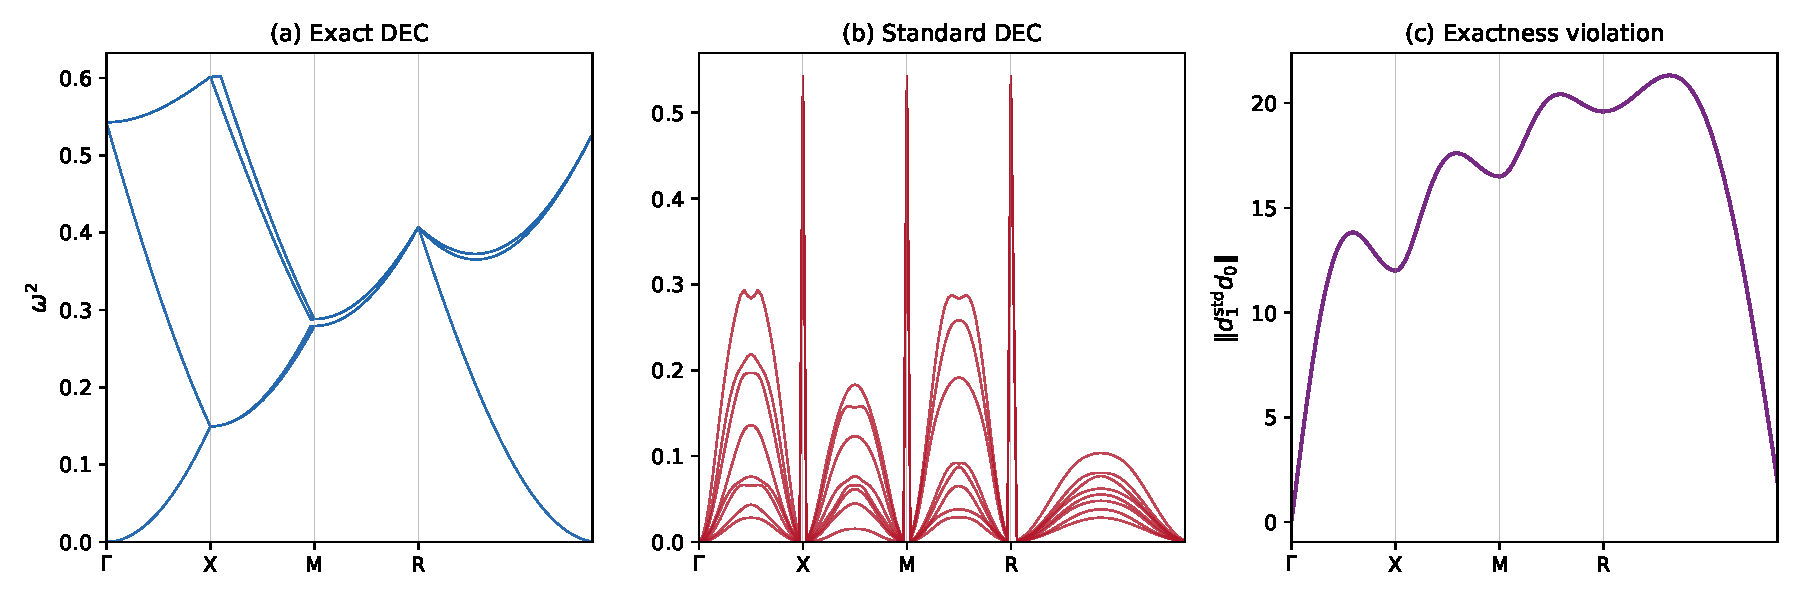
\includegraphics[width=\textwidth]{fig3_bands.pdf}
\caption{Band structure along $\Gamma$--X--M--R--$\Gamma$ for Kelvin $N{=}2$.
(a)~Exact DEC: clean bands with twofold acoustic degeneracy near~$\Gamma$.
(b)~Standard DEC: spurious bands collapse toward zero at high-symmetry points;
the first non-zero eigenvalue is a spurious mode, not acoustic.
(c)~Exactness violation $\|d_1^{\mathrm{std}} d_0\|$: grows from~0 at~$\Gamma$
to~$\sim 20$ at~R, confirming that the failure is $O(|\kk|)$.}
\label{fig:bands}
\end{figure}

% ============================================================
\section{Consequences of inexactness}
\label{sec:inexactness}
% ============================================================

Three structural results explaining the spectral pathology of
\S\ref{sec:spectral}. These connect the curvature structure of
\S\ref{sec:construction} (local phase inconsistency on each face) to the
global spectral consequences.

\subsection{Rank--pollution identity}

\begin{proposition}[Rank--pollution identity]\label{prop:rank}
$\rank(d_1^{\mathrm{std}}) - \rank(d_1^{\mathrm{ex}}) = n_{\mathrm{spur}}$.
\end{proposition}

\begin{proof}
Both $d_1^{\mathrm{ex}}$ and $d_1^{\mathrm{std}}$ have identical sparsity
patterns and unimodular entries. They differ only in phases. On the exact
complex, $\cker K = \cker d_1$ has dimension~$|V|$
(Proposition~\ref{prop:kernel}). On the standard complex, $\cker K_{\mathrm{std}}$
has dimension $|V| - n_{\mathrm{spur}}$. Since $\cker K = \cker d_1$ when
$\star_2 > 0$, the kernel dimension change equals the rank change:
$\dim\cker d_1^{\mathrm{std}} - \dim\cker d_1^{\mathrm{ex}} = -n_{\mathrm{spur}}$,
hence $\rank(d_1^{\mathrm{std}}) - \rank(d_1^{\mathrm{ex}}) = n_{\mathrm{spur}}$.
\end{proof}

Verified on all structures and all $\kk$-directions:
Kelvin $[100]$: $102 - 96 = 6 = n_{\mathrm{spur}}$;
$[110]$: $108 - 96 = 12$;
$[111]$: $110 - 96 = 14$.

\subsection{Hodge hybridization at random baseline (empirical)}

On exact DEC: gauge modes have gradient overlap~1.000, physical modes~0.000.
On standard DEC: spurious modes have overlap 0.514~(Kelvin), 0.524~(C15),
0.513~(WP)---within 3\% of the random baseline $|V|/|E| = 0.500$. The
spurious modes show no statistically significant deviation from random
gradient/curl content. The failure is in the deep non-perturbative regime,
not a small correction.

\subsection{Trace conservation}

$\tr(M^{-1}K)$ is identical for exact and standard DEC:
\[
  \mathrm{rel\_diff} < 1.78 \times 10^{-16} \quad \text{across 5 $\kk$-directions.}
\]
This is a topological invariant: $|d_1[f,e]| = 1$ for both constructions on
the same support, so the trace depends only on the incidence structure and
Hodge stars, not on the phases. Consequence: spurious eigenvalues cannot simply
appear from nothing---they must be compensated by shifts in physical
eigenvalues. The spectral damage is redistributed, not created.

% ============================================================
\section{Application: Voronoi tessellations}
\label{sec:voronoi}
% ============================================================

The exact construction enables identification of geometries where the
curl--curl operator has optimal spectral properties.

\subsection{Metric isotropy}

\begin{property}[Voronoi isotropy]\label{prop:voronoi}
On periodic Voronoi tessellations of~$T^3$, we observe that the discrete
metric tensors satisfy $G = \Vol \cdot I$ and $H = \Vol \cdot I$.
\end{property}

The identity can be understood via the divergence theorem on dual cells
(for~$G$) and primal cells (for~$H$), exploiting the perpendicularity of
Voronoi edges and dual faces. A complete proof is provided in the
Supplementary Material (Section~S1).

\emph{Verified:} $\|G/\Vol - I\| < 10^{-15}$ on cubic structures,
$< 5 \times 10^{-12}$ on random Voronoi (5~seeds). Robust under
near-degeneracy: with generators clustered within $\delta = 0.01$
($\min\star_1 = 3.5 \times 10^{-5}$), the identity holds at
$3.5 \times 10^{-12}$.

\subsection{Exact dispersion}

Metric isotropy combined with Theorem~\ref{thm:existence} (exactness) yields:
\begin{equation}\label{eq:dispersion}
  \omega^2 = |\kk|^2 + O(|\kk|^4).
\end{equation}
The argument proceeds by Schur complement reduction of~$K(\kk)$ onto the 3D
harmonic subspace at~$\Gamma$; exactness ensures this subspace is well-defined
(Proposition~\ref{prop:kernel}), and $G = H = \Vol\cdot I$ makes the effective
operator proportional to $|\kk|^2 I$. Full derivation in Supplementary
Material (Section~S2).

\emph{Verified:} $c^2 = 0.9993$--$0.9997$ on cubic structures,
$0.9995$--$0.9996$ on random Voronoi (5~seeds). Standard DEC:
$c^2_{\mathrm{std}} = 0.52$--$1.55$ (spurious, not acoustic). Both metric
tensors matter: perturbing~$\star_2$ gives $\Delta c^2 = 0.024$,
perturbing~$\star_1$ gives $\Delta c^2 = 0.012$. Neither alone is sufficient.

Full spectral analysis, including the converse and moment conservation,
in~[Paper~A2].

% ============================================================
\section{Discussion}
\label{sec:discussion}
% ============================================================

\paragraph{Comparison with finite elements}
A quantitative comparison with N\'ed\'elec edge elements on the same eigenvalue
problems is not included in this work. Such a comparison---measuring $L^2$ and
$H(\mathrm{curl})$ errors on standard benchmark problems---would situate the
DEC construction relative to established FEEC methods and is planned for a
companion study.

\paragraph{Limitations}
The Hodge stars are diagonal (circumcentric dual); non-diagonal stars would
require modification of the assembly but not the exactness construction. The
mesh must have valid polyhedral structure; for random Voronoi, sufficient point
density is required ($\geq 50$ points per periodic box gives $> 80\%$ valid
tessellations). The construction is lowest-order (piecewise-constant cochains);
extension to higher-order DEC would require a corresponding generalization of
the recurrence. The observed $O(1/N^2)$ convergence rate is consistent with a
lowest-order discretization but a formal error estimate is not attempted.

\paragraph{Open questions}
\begin{itemize}
  \item Non-flat connections (magnetic flux): the recurrence requires
    $H_f = 1$ (flat holonomy). For $F \neq 0$, a modified recurrence is an
    open mathematical problem.
  \item Non-abelian gauge: matrix-valued $d_0/d_1$ infrastructure not yet
    available.
  \item Non-$T^3$ topology: lens spaces, Seifert manifolds require different
    mesh builders.
  \item Converse of Voronoi optimality ($c^2 = 1$ implies metric isotropy) and
    moment conservation $\to$ [Paper~A2].
  \item 2D validation with photonic crystal benchmarks $\to$ [Paper~B].
\end{itemize}

% ============================================================
\section{Conclusion}
\label{sec:conclusion}
% ============================================================

The standard Bloch-periodic extension of DEC does not preserve the discrete
exact sequence on unstructured polyhedral meshes. This structural failure
produces spectral pollution, destroys the Hodge decomposition, and prevents
convergence. A face-boundary recurrence restores exactness by deriving curl
phases from those in the gradient, producing a canonical curl--curl operator
with correct gauge kernel. The construction extends to the full cochain complex
($d_2 d_1 = 0$) and computes the correct twisted de~Rham cohomology. On
periodic Voronoi tessellations, exactness combined with metric isotropy yields
exact isotropic wave speed. The failure is algebraic---independent of mesh
quality, resolution, or symmetry---and is confirmed on five qualitatively
different polyhedral complexes including random Voronoi meshes with no symmetry.

% ============================================================
\section*{Reproducibility}
% ============================================================

All computations use Python~3.9+ with NumPy~1.24+ and SciPy~1.11+. Source code
and complete test suite available at
\url{https://github.com/alex-toader/st_exact_deRham}.

\paragraph{Test suite} 57~tests organized in 7~files mirroring the paper
structure:

\begin{table}[h]
\centering\small
\begin{tabular}{llrl}
\toprule
File & \S & Tests & What \\
\midrule
\texttt{test\_01\_setup}           & 2   & 6  & Structure, Euler $\chi$, Hodge stars \\
\texttt{test\_02\_standard\_fails} & 3   & 12 & Failure, Cor~1, scaling, sensitivity \\
\texttt{test\_03\_recurrence}      & 4   & 14 & Thm~1, holonomy, uniqueness, kernel \\
\texttt{test\_04\_spectral\_gains} & 5   & 8  & Pollution, Hodge, convergence \\
\texttt{test\_05\_inexactness}     & 6   & 3  & Rank identity, hybridization, trace \\
\texttt{test\_06\_voronoi}         & 7   & 8  & Isotropy, $c^2{=}1$, near-degeneracy \\
\texttt{test\_07\_curvature}       & 4/6 & 5  & Curvature, flux, cancellation \\
\bottomrule
\end{tabular}
\end{table}

Total runtime: $\sim$70s on a single core. Each test file includes expected
output in its header docstring for comparison. The mapping from test~ID to
paper claim is documented in \texttt{tests/tests\_map.md}.

\paragraph{Running} From the project root:
\begin{verbatim}
python3 run_tests.py                    # all tests
python3 run_tests.py recurrence voronoi # specific groups
\end{verbatim}

\paragraph{Structures} Five test structures are used throughout: SC cubic
($N{=}3$), three periodic Voronoi tessellations (Kelvin/BCC $N{=}2$,
C15/Laves $N{=}1$, Weaire--Phelan/A15 $N{=}1$), and random periodic Voronoi
(10~seeds, $n{=}50$ cells). Structure builders are deterministic given seed
and size parameters.


% ============================================================
% References
% ============================================================
\begin{thebibliography}{99}

\bibitem{Arnold2006}
D.~N. Arnold, R.~S. Falk, R.~Winther,
Finite element exterior calculus, homological techniques, and applications,
\textit{Acta Numer.}~\textbf{15} (2006) 1--155.

\bibitem{Arnold2010}
D.~N. Arnold, R.~S. Falk, R.~Winther,
Finite element exterior calculus: from Hodge theory to numerical stability,
\textit{Bull.\ Amer.\ Math.\ Soc.}~\textbf{47} (2010) 281--354.

\bibitem{Boffi2010}
D.~Boffi,
Finite element approximation of eigenvalue problems,
\textit{Acta Numer.}~\textbf{19} (2010) 1--120.

\bibitem{Boffi2006}
D.~Boffi, M.~Conforti, L.~Gastaldi,
Modified edge finite elements for photonic crystals,
\textit{Numer.\ Math.}~\textbf{105} (2006) 249--266.

\bibitem{Bossavit1998}
A.~Bossavit,
\textit{Computational Electromagnetism},
Academic Press, 1998.

\bibitem{BottTu1982}
R.~Bott, L.~W. Tu,
\textit{Differential Forms in Algebraic Topology},
Springer, 1982.

\bibitem{Hatcher2002}
A.~Hatcher,
\textit{Algebraic Topology},
Cambridge University Press, 2002.
(Chapter~3.H: Cohomology with local coefficients.)

\bibitem{Christiansen2008}
S.~H. Christiansen,
A construction of spaces of compatible differential forms on cellular complexes,
\textit{Math.\ Models Methods Appl.\ Sci.}~\textbf{18} (2008) 739--757.

\bibitem{Desbrun2005}
M.~Desbrun, A.~N. Hirani, M.~Leok, J.~E. Marsden,
Discrete exterior calculus,
\texttt{arXiv:math/0508341} (2005).

\bibitem{DiPietro2020}
D.~A. Di~Pietro, J.~Droniou,
\textit{The Hybrid High-Order Method for Polytopal Meshes},
Springer, 2020.

\bibitem{Hiptmair2002}
R.~Hiptmair,
Finite elements in computational electromagnetism,
\textit{Acta Numer.}~\textbf{11} (2002) 237--339.

\bibitem{Hirani2003}
A.~N. Hirani,
\textit{Discrete Exterior Calculus},
PhD thesis, California Institute of Technology, 2003.

\bibitem{Monkola2023}
S.~M\"onk\"ol\"a, J.~Räbinä, T.~Rossi,
Discrete exterior calculus for photonic crystal waveguides,
\textit{Int.\ J.\ Numer.\ Meth.\ Eng.}~\textbf{124} (2023) 1035--1054.

\bibitem{Schulz2018}
J.~Schulz, K.~Taixeira,
Numerical electromagnetic frequency domain analysis with discrete exterior calculus,
\textit{J.\ Comput.\ Phys.}~\textbf{350} (2017) 497--519.

\bibitem{Teixeira1999}
F.~L. Teixeira, W.~C. Chew,
Lattice electromagnetic theory from a topological viewpoint,
\textit{J.\ Math.\ Phys.}~\textbf{40} (1999) 169--187.

\end{thebibliography}

\end{document}
